\documentclass[../m136main.tex]{subfiles}
\graphicspath{{\subfix{../figures/}}}

\begin{document}

\chapter{Residue Theory}
\section{Computing Residues}
We'll spend the next while seeing how the theory of contour integrals can be leveraged to evaluate integrals over the real numbers.
Our discussion will center around the following definition and theorem.

\begin{definition}[Residue]
    If $f(z)$ has an isolated singularity at $z_0 \in \C$ then the coefficient $c_{-1}$ of $(z - z_0)^{-1}$ in its Laurent series about $z_0$ is called the residue of $f$ at $z_0$; it is denoted $\Res(f; z_0)$.
\end{definition}

\begin{theorem}[The residue theorem]
    Let $\Gamma$ be a simple closed positively-oriented curve, and let $f$ be analytic on $\Gamma$.
    If $\Gamma$ is also analytic inside $\Gamma$, except potentially at isolated singularities $z_1, \, \ldots, \, z_N$, then
    \[ \oint_\Gamma f(z) \,dz = 2\pi i \sum_{k=1}^{N} \Res(f; z_k). \]
\end{theorem}

\begin{proof}
    We can deform $\Gamma$ into a collection of small circles $\gamma_k$ surrounding each singularity, all connected by twice-traversed lines.
    Thus
    \[ \oint_\Gamma f(z) \,dz = \sum_{k=1}^{N} \oint_{\gamma_k} f(z) \,dz = 2\pi i \sum_{k=1}^{N} \Res(f; z_k), \]
    as desired.
\end{proof}

Thankfully, we don't need to actually compute the Laurent series of a function in order to determine its residues.
If $f$ has a simple pole at $z_0$ then we can simply write
\[ (z - z_0) f(z) = c_{-1} + c_0(z - z_0) + \cdots, \]
where $c_k$ are the terms of the Laurent series of $f$ about $z_0$.
We can make all of the non-$c_{-1}$ terms vanish by taking $z \to z_0$.

\begin{lemma}[Useful lemma]
    If $f$ has a simple pole at $z_0$ then
    \[ \Res(f; z_0) = \lim_{z \to z_0} (z - z_0) f(z). \]
\end{lemma}

\begin{lemma}[Very useful lemma]
    If $f(z) = P(z) / Q(z)$ with $P,Q$ analytic, $Q(z)$ has a simple pole at $z_0$, and $P(z_0) \neq 0$, then
    \[ \Res(f; z_0) = \frac{P(z_0)}{Q'(z_0)}. \]
\end{lemma}

\begin{proof}
    By the previous lemma,
    \begin{align*}
        \Res(f; z_0) &= \lim_{z \to z_0} \frac{P(z)}{Q(z) - 0} \\
        &= \lim_{z \to 0} \frac{P(z)}{[Q(z) - Q(z_0)] / (z - z_0)} \\
        &= \frac{P(z_0)}{Q'(z_0)},
    \end{align*}
    as desired.
\end{proof}

If we have a pole of order $N$ we can take a similar approach by first multiplying by $(z - z_0)^{N}$ to get
\[ (z - z_0)^{N} f(z) = c_{-N} + \cdots + c_{-1} (z - z_0)^{N-1} + \cdots, \]
and then we can take a bunch of derivatives to peel off the $c_{-1}$ coefficient.

\begin{theorem}[]
    If $f(z)$ has a pole of order $N$ at $z_0$ then
    \[ \Res(f; z_0) = \frac{1}{(N-1)!} \lim_{z \to z_0} \frac{d^{N-1}}{dz^{N-1}} \left[ \left( z - z_0 \right)^{N} f(z) \right]. \]
\end{theorem}

For an essential singularity there is, unfortunately, no nice formula---we just need to ``massage out'' the sum.
Now we'll go through a bunch of examples, each of which illustrates a different technique for evaluating real integrals using residues.

\begin{example}[Parametrization]
    We'd like to evaluate
    \[ I = \int_{0}^{2\pi} \frac{1}{1 + a^2 - 2a \cos \theta} \,d\theta, \qquad a > 0, \quad a \neq 1. \]
    The bounds here suggest that we make the substitution  $z = e^{i\theta}$, $\theta \in [0,2\pi]$:
    \begin{align*}
        I &= \oint_{|z| = 1} \frac{1}{1 + a^2 + 2a [(z + 1 / z) / 2]} \frac{dz}{iz} \\
        &= i \oint_{|z| = 1} \frac{1}{(az - 1)(z - a)} \,dz.
    \end{align*}
    The integrand has simple poles at $z = a$ and $z = 1 / a$, so technically speaking we have two cases: $0 < a < 1$ and $a > 1$.
    In both cases, though, the residues are
    \[ \Res(f; a) = \frac{1}{a^2 - 1}, \]
    and since exactly one of these singularities is in the contour we get
    \[ I = \frac{2\pi}{|1 - a^2|}. \]
\end{example}

We should quickly note that, strictly speaking, integrals over singularities do not exist.
What we've actually done here is determine the ``principal value'' of the integral---if $f$ has an isolated singularity at $x_0 \in (a,b)$, then
\[ \textrm{p.v.} \int_{a}^{b} f(x) \,dx = \lim_{\varepsilon \to 0} \left[ \int_{a}^{x_0 - \varepsilon} f(x) \,dx + \int_{x_0 + \varepsilon}^{b} f(x) \,dx \right]. \]
We're only concerned with the principal values of our integrals here, so we'll continue to omit the \textrm{p.v.}


\section{Improper Integrals via Contour Closure}
A very common technique for evaluating improper integrals in $\R$ is to imagine the line we're integrating over as one piece of a very large, closed contour.
The next few examples will show how we choose such a contour.

\begin{example}[A semicircle]
    We'd like to confirm that
    \[  \int_{-\infty}^{\infty} \frac{1}{1 + x^2} \,dx = \pi. \]
    To do this we construct a closed contour $\Gamma_C = \Gamma_1 + \Gamma_R$, where $\Gamma_1$ is the segment of the real line $(-R, R)$ with $R > 1$, and $\Gamma_R$ is the upper semicircle which closes the contour.
    \begin{itemize}[topsep=0pt]
        \item An application of the residue theorem shows that the integral over $\Gamma_C$ is $I_C = \pi$.
        
        \item Rather than precisely determining the $\Gamma_R$ contribution $I_R$, we'll just determine an upper bound.
        By the lower triangle inequality we have $|1 + z^2| \geq \left| |1| - |z|^2 \right| = |1 - R^2|$, so by the ML lemma
        \[ |I_R| \leq \frac{1}{R^2 - 1} \cdot \pi R. \]
    \end{itemize}   \vspace{-6pt}
    The integral we seek is therefore
    \[ \int_{-\infty}^{\infty} \frac{1}{1 + x^2} \,dx = \lim_{R \to \infty} (I_C - I_R) = \pi - 0 = \pi. \]
    Conveniently, the contribution from the semicircular part of our contour vanishes completely, leaving us just with the $\pi$ we desired!
    (The same method works for integrands like $x^2 / (1 + x^{4})$.)
\end{example}

\begin{example}[A rectangle]
    We'd like to evaluate
    \[ \int_{-\infty}^{\infty} \frac{e^{ax}}{1 + e^{x}}, \quad a \in (0,1). \]
    Due to the structure of the singularities, rather than using a semicircle (which encloses an increasing number of singularities as it grows), we should use an expanding rectangle with fixed height $2\pi$.
    \begin{itemize}[topsep=0pt]
        \item By the residue theorem, the integral over the closed contour is $-2\pi i e^{a\pi i}$.
        
        \item We parametrize the rightmost piece using $z(t) = R + it$, $t \in [0, 2\pi]$ and bound it using the ML lemma.
        The contribution of this piece vanishes as $R \to \infty$; the same goes for the leftmost piece.

        \item For the topmost piece, which we call $\Gamma_T$ we parametrize $z(t) = t + 2\pi i$, $t \in [-R, R]$.
        After some algebra, this yields
        \[ \int_{\Gamma_3} \frac{e^{az}}{1 + e^{z}} \,dz = -e^{2\pi a i} \int_{\Gamma_1} f(z) \,dz, \]
        where $\Gamma_1$ is the bottommost piece (on the real line).
    \end{itemize}
    Putting all this together, the integral turns out to be
    \[ \int_{-\infty}^{\infty} \frac{e^{ax}}{1 + e^{x}} = \frac{-2\pi i e^{a\pi i}}{1 - e^{2\pi a i}} = -\frac{2\pi i}{e^{-a\pi i} - e^{a\pi i}} = \frac{\pi}{\sin a\pi}. \]
\end{example}

\begin{example}[A pizza slice]
    We'd like to evaluate
    \[ \int_{0}^{\infty} \frac{1}{x^3} \,dx. \]
    To avoid putting a singularity on our path, we'll integrate over a ``pizza slice'' contour---a segment on $[0,R]$ connects with a circular arc of $2\pi / 3$ radians, which connects to the origin via another segment.
    \begin{itemize}[topsep=0pt]
        \item By the residue theorem, the integral over the entire slice is $e^{-i(2\pi / 3)} / 3$.
        
        \item For the arc we impose a bound that vanishes as $R \to \infty$.
        
        \item For the diagonal ray we parametrize $t e^{i(2\pi / 3)}$ and do some algebra to get
        \[ \int_{\Gamma_D} \frac{1}{1 + z^3} \,dz = -e^{i(2\pi / 3)} \int_{0}^{R} \frac{1}{1 + z^3} dz. \]
    \end{itemize}
    Thus the integral is
    \[ \int_{0}^{\infty}\frac{1}{1 + z^3} \,dz = \frac{2\pi i}{3e^{i(2\pi / 3)}} \frac{1}{1 - e^{i(2\pi / 3)}} = \frac{2i\pi / 3}{e^{i(2\pi / 3)} - e^{-i(2\pi / 3)}} = \frac{2\pi}{3 \sqrt{3}}. \]
\end{example}

\begin{example}[Forcing a semicircle]
    We'd like to evaluate
    \[ \int_{-\infty}^{\infty} \frac{\cos x}{x^2 + a^2} \,dx = \Re \left[ \int_{-\infty}^{\infty} \frac{e^{ix}}{x^2 + a^2} \,dx \right], \qquad a > 0. \]
    We can't immediately use a semicircle since the cosine is exponential on the imaginary axis, but if we frame the integral as the real part of another expression the problem becomes tractable!
    \begin{itemize}[topsep=0pt]
        \item By the residue theorem, the closed integral is $\pi / (ae^{a})$.
        \item On the semicircular bit we put a vanishing bound on the integral.
        \item Integrating the $i \sin x$ term on the real line gives zero, since it produces an odd function.
    \end{itemize}
    Putting it all together, the integral we seek is $\pi / a e^{a}$.
\end{example}

\section{Some Useful Lemmas}
Now we'll detour for a bit and look at some general statements that'll be useful in evaluating more integrals.

\begin{lemma}[Jordan's lemma]
    If $C_R^+$ denote the upper half of a radius-$R$ circle centered at 0 then
    \[ \left| \int_{C_R^+} e^{iz} \,dz \right| < \pi. \]
\end{lemma}


\begin{proof}
    By parametrization,
    \begin{align*}
        \left| \int_{C_R^+} e^{iz} \,dz \right| &= \left| \int_{0}^{\pi} e^{iR e^{it}} iR e^{it} \,dt \right| \\
        &\leq R \int_{0}^{\pi} e^{-R \sin t} \,dt \\
        &= 2R \int_{0}^{\pi / 2} e^{-R \sin t} \,dt. \\
        \intertext{Note that $\sin t \geq (2 / \pi) t$ for $t \in [0, \pi]$, meaning}
        &\leq 2R \int_{0}^{\pi / 2} e^{-R (2 / \pi) t} \,dt < \pi
    \end{align*}
    for all $R > 0$, as desired.
\end{proof}

\begin{lemma}[Fancy Jordan lemma]
    Let $\ds M(r) = \max_{z \in C_R^+} |f(z)|$. \vspace{-12pt}
    If $\ds \lim_{R \to \infty} M(R) = 0$ then for all $m > 0$,
    \[ \lim_{R \to \infty} \int_{C_R^+} f(z) e^{i m z} dz = 0. \]
\end{lemma}

\begin{proof}
    Like before, we parametrize:
    \begin{align*}
        \left| \int_{C_R^+} f(z) e^{imz} dz \right| &\leq \int_{0}^{\pi} |f(Re^{it})| |e^{im R e^{it}}| |i R e^{it}| dt \\
        &\leq \int_{0}^{\pi} M(R) e^{-m R \sin t} R \,dt \\
        &\leq 2 R \, M(R) \int_{0}^{\pi / 2} e^{-mR(2 / \pi) t} \,dt \\
        &= \frac{\pi M(R)}{m} (1 - e^{-mR}),
    \end{align*}
    which vanishes as $R \to \infty$.
\end{proof}

Note that we may apply this lemma to any rational integrand whose numerator is of lower degree than its denominator.
We have one more lemma before jumping back into examples---note the similarities with the residue theorem.

\begin{lemma}[]
    Let $f(z)$ have a simple pole at $z_0$ and let $\Gamma_R$ be the arc $z = z_0 + R e^{it}$, $t \in [0, \alpha]$.
    Then
    \[ \lim_{R \to 0} \int_{\Gamma_R} f(z) \,dz = \alpha i \Res(f; z_0). \]
\end{lemma}

\begin{proof}
    Since $z_0$ is a simple pole, there exists an $\varepsilon > 0$ and an analytic $h(z)$ such that
    \[ f(z) = \frac{c_{-1}}{z - z_0} + h(z). \]
    So for $0 < R < \varepsilon$ we have
    \[ \int_{\Gamma_R} f(z) \,dz = c_{-1} \int_{\Gamma_R} \frac{dz}{z - z_0} + \int_{\Gamma_R} h(z) \,dz, \]
    Since $h(z)$ is bounded on $B(z_0, \varepsilon)$, by the ML lemma the second integral vanishes as $R \to 0$.
    Parametrization reveals that the first term is $c_{-1}(\alpha i)$, meaning the overall integral is $\alpha i \Res(f; z_0)$, as desired.
\end{proof}

\pagebreak

\section{More Examples}
Now we'll look at some more instructive examples.

\begin{example}[A semicircle with a bump]
    We'd like to evaluate
    \[ \int_{-\infty}^{infty} \frac{\cos 2x}{1 + x} \,dx = \Re \left[ \int_{-\infty}^{\infty} \frac{e^{2ix}}{1 + x} \,dx \right]. \]
    We'll once again use a semicircle, but this time accented with a small semicircular bump at $z=1$.
    \begin{itemize}[topsep=0pt]
        \item By the fancy Jordan lemma, the integral over the large semicircle vanishes as $R \to \infty$.
        \item By the previous lemma, the integral over the small semicircle goes to $-\pi i e^{-2i}$ as $\varepsilon \to 0$.
    \end{itemize}
    The other two pieces comprise the integral we care about (as $\varepsilon \to 0$), meaning
    \[ \int_{-\infty}^{\infty} \frac{\cos 2x}{1 + x} \,dx = \Re \left[ \pi i e^{-2i} \right] = \pi \sin 2. \]
\end{example}

\begin{example}[Deriving a sum]
    The function $f(z) = \pi \cot \pi z$ has simple poles at every $z = k \in \Z$, since it is of the form $h'(z) / h(z)$; defining $g(z) = f(z) / z^2$ turns the singularity at $k=0$ into a pole of order 3.
    The residues for $k \neq 0$ are $1 / k^2$, and that for $k = 0$ is $-\pi^2 / 3$.

    Consider the contour $\Gamma_k$, a square centered at the origin which intersects the axes at $x,y = \pm (k + 1 / 2)$.
    By expressing $\cot \pi z$ in terms of complex exponentials, we could show that
    $|\cot \pi z| \leq 1$ and $|\cot \pi z| \leq 2$ on the vertical and horizontal paths, respectively.
    Using these,
    \[ \left| \oint_{\Gamma_k} \frac{\pi \cot \pi z}{z^2} \,dz \right| \leq \frac{2\pi}{(k + 1 / 2)^2} \cdot 4(2k + 1) \longrightarrow \, 0, \]
    and so
    \[ 0 = 2\pi i \cdot \sum_{k=-\infty}^{\infty} \Res(g; k) = 2\pi i \left( 2 \sum_{k=1}^{\infty} \frac{1}{k^2} - \frac{\pi^2}{3} \right) \;\implies\; \sum_{k=1}^{\infty} = \frac{\pi^2}{6}. \]
    But the Laurent expansion of $\pi \cot (\pi z) / z^2$ has a nonzero term for every even power of $z$, so this is a geneal method for generating values of $\sum_{k=1}^{\infty} k^{-2n}$.
\end{example}

\begin{example}[A keyhole]
    \parbox{0.62\textwidth}{
        We'd like to evaluate
        \[ I = \int_{0}^{\infty} f(x) \,dx, \qquad f(x) = \frac{1}{x^{1 / 3}(x+2)}. \]
        Perhaps contrary to what our intuition would tell us, we'll put the branch cut on the axis we're integrating over so that $\log(z) = \Log_0(z)$.
        We'll use the ``keyhole'' contour $\Gamma_\varepsilon^\delta$ drawn at right.
        It is comprised of four pieces: two almost-circles $\gamma_R^\delta, \gamma_\varepsilon^\delta$ and two segments $\gamma_1^\delta, \gamma_2^\delta$ connecting their loose ends.
        \vspace{6pt}

        There's a simple pole at $z = -2$, so by the residue theorem the integral about $\Gamma_\varepsilon^\delta$ is $2\pi i / (2^{1 / 3} e^{i(\pi / 3)})$.
        Now for the pieces.
    }\parbox{0.38\textwidth}{
        \quad\;
        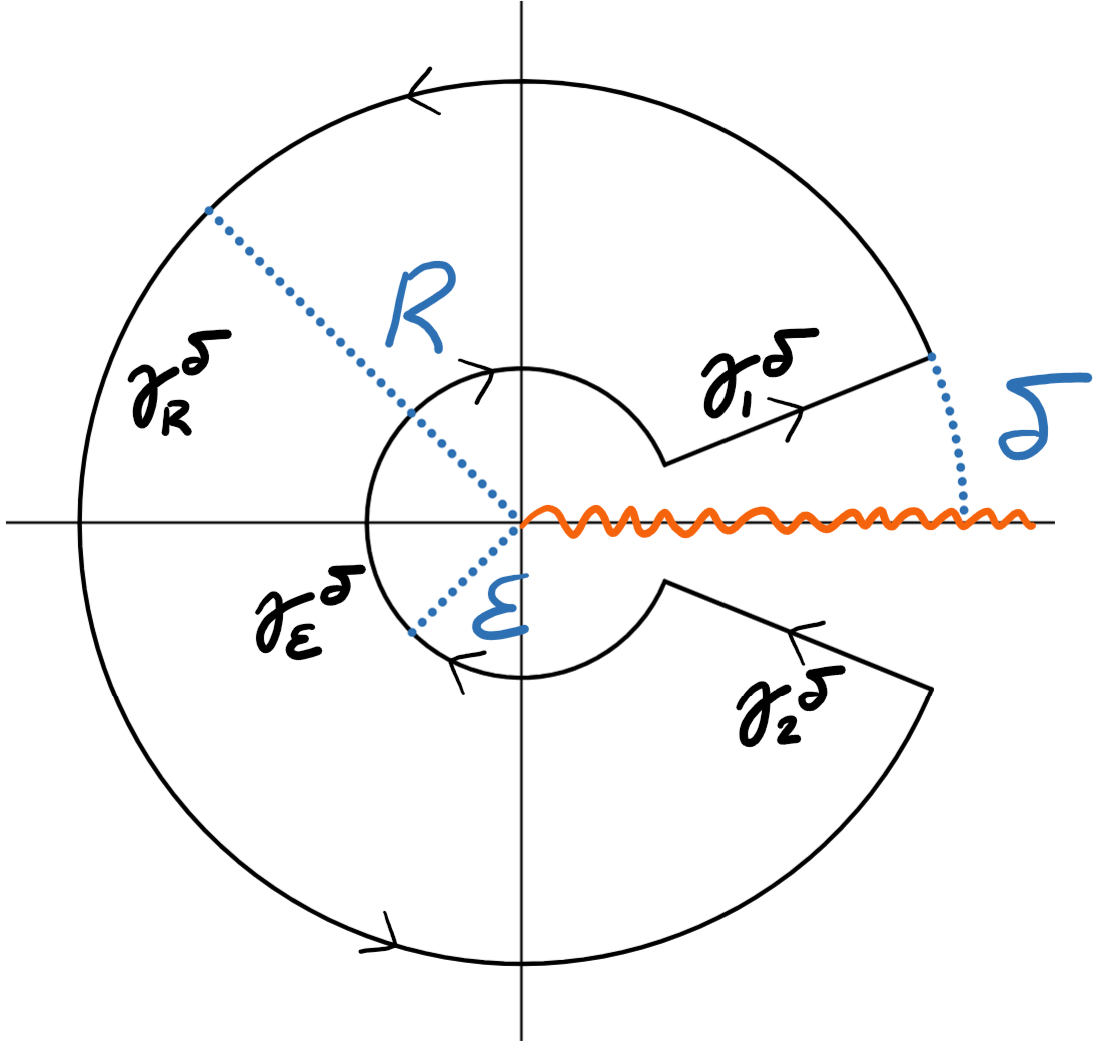
\includegraphics[width=0.34\textwidth]{keyhole.png}
    }

    \begin{itemize}[topsep=0pt]
        \item We put bounds on the integrals over $\gamma_R^\delta$ and $\gamma_\varepsilon^\delta$ which vanish as $R \to \infty$ and $\varepsilon \to 0$.
        
        \item $\gamma_1^\delta$ is parametrized by $t e^{i\delta}$, $t \in [\varepsilon, R]$, so $z^{1 / 3} = t^{1 / 3} e^{i(\delta / 3)}$ and as $\delta \to 0$ we get $z^{1 / 3} \to t^{1 / 3}$.
        Similarly, $-\gamma_2^\delta$ is parametrized by $te^{i(2\pi - \delta)}$, $t \in [\varepsilon, R]$.
        Like before, we get $z^{1 / 3} \to t^{1 / 3} e^{i(2\pi / 3)}$.
    \end{itemize}
    What we've done here is show that
    \[ \lim_{\delta \to 0^+} \int_{\gamma_1^{\delta}}^{} f(z) \,dz = \int_{\varepsilon}^{R} \frac{dx}{x^{1 / 3}(x+2)}, \quad \lim_{\delta \to 0^+} \int_{\gamma_2^{\delta}}^{} f(z) \,dz = -e^{-i (2\pi / 3)} \int_{\varepsilon}^{R} \frac{dx}{x^{1 / 3}(x+2)}. \]
    Summing all these pieces' contributions together gives
    \[ \lim_{\substack{\delta,\varepsilon \to 0^{+} \\ R \to \infty}} \oint_{\Gamma_\varepsilon^\delta} f(z) \,dz = (1 - e^{-i (2\pi / 3)}) \int_{0}^{\infty} \frac{dz}{x^{1 / 3} (x+2)} = \frac{2\pi i}{2^{1 / 3} e^{i(\pi / 3)}}, \]
    meaning
    \[ \int_{0}^{\infty} \frac{dz}{x^{1 / 3} (x+2)} = \frac{2\pi i}{2^{1 / 3} e^{i(\pi / 3)}} \frac{1}{1 - e^{-i(2\pi / 3)}} = \frac{\pi}{\sqrt[3]{2}} \frac{1}{\sin(\pi / 3)} = \frac{2^{2 / 3} \pi}{\sqrt{3}}. \]
\end{example}

This integral is a special case of a more general integral transform.

\begin{definition}[Mellin transform]
    The Mellin transform of $f : [0, \infty) \to \R$ is
    \[ \mathcal M[f](a) = \int_{0}^{\infty} x^{a - 1} f(x) \,dx, \qquad a \in \C, \]
    provided the limit exists.
\end{definition}

Notice that the Mellin transform of $f(t) = e^{-t}$ is the gamma function $\Gamma(z)$!
This function is well-defined and analytic for all $\Re(z) > 0$ (since $x-1 > -1$ for integrability), and notably it satisfies $\Gamma(z+1) = z \, \Gamma(z)$ (so $\Gamma(n+1) = n!$).

We can repeatedly use this property to extend the domain of $\Gamma$ to all of $\C$, barring simple poles at the negative integers.
For example, to extend the domain to all $\Re(z) > -m$ we'd write
\[ F_m(z) = \frac{\Gamma(z+m)}{z(z+1)(z+2) \cdots (z+m-1)}. \]
With this, we could show that $\Res(-k) = (-1)^{k} / k!$.
(We could do a similar ``analytic continuation'' with the zeta function $\zeta(z)$, but that involves a messier functional equation.)
There's lots of interesting stuff to be seen with the gamma function, but it's time to move on now.

\section{The Laplace Transform}
Now we'll take a closer look at a more familiar transform.

\begin{definition}[Laplace transform]
    The Laplace transform of $f : [0,\infty) \to \C$ is
    \[ \mathcal L[f](z) = F(z) = \int_{0}^{\infty} e^{-zt} f(z) \,dt, \]
    provided this limit exists.
\end{definition}

When working with the Laplace transform we work specifically with the class of exponential functions, those satisfying $|f(t)| < A e^{Bt}$ for some $A > 0$, $B \in \R$, and $t \geq 0$.
We put further restrictions on these parameters:
\[ |F(z)| \leq \int_{0}^{\infty} |f(t)| e^{-\Re(z) t} \,dt \leq A \int_{0}^{\infty} e^{(B - \Re z)t} \,dt = \frac{A}{\Re z - B}. \]
For this inequality to work out, we require $\Re z > B$.
Now, usually at this point we'd go through and compute a bunch of sample transforms and maybe use them to solve some differential equations, but we'll note only that the transforms of derivatives look like
\begin{align*}
    \mathcal L[f'] (z) &= z \mathcal L[f](z) - f(0), \\
    \mathcal L[f''] (z) &= z^2 \mathcal L[f](z) - z f(0) - f'(0),
\end{align*}
and so on, and then jump straight into inverses.

\begin{definition}[Inverse Laplace transform]
    Given $F(z)$ with finitely many isolated singularities, we define
    \[ \mathcal L^{-1}[F(z)](t) = \frac{1}{2\pi i} \int_{\alpha - i\infty}^{\alpha + i\infty} F(z) \,e^{zt} \,dt \]
    with $\alpha \in \R$ chosen so that all singularities lie to the left of $\alpha$.
\end{definition}

This can get messy, but there's an incredibly nice formula for evaluating inverse Transforms for many functions.

\begin{theorem}[]
    If $F(z)$ is analytic on $\C$ except at finitely many isolated singularities $z_k$, if $\ds \lim_{z \to \infty} F(z) = 0$ then  \vspace{-6pt}
    \[ \mathcal L^{-1}[F(z)](t) = \sum_{z_k}^{} \Res(e^{zt} F(z); z_k). \]
\end{theorem}

\begin{proof}
    Our assumptions about $F$ imply that there exists some $\sigma \in \R$ such that $F(z)$ is analytic for all $\Re z > \sigma$.
    For any $\alpha > \sigma$, by definition
    \begin{align*}
        \mathcal L^{-1}[F(z)](t) &= \frac{1}{2\pi i} \int_{\alpha - i\infty}^{\alpha + i\infty} e^{zt} F(z) \,dz \\
        &= \frac{1}{2\pi i} \left[ 2\pi i \sum_{z_k}^{} \Res \left( e^{zt} F(z); z_k \right) \right] \\
        &= \sum_{z_k}^{} \Res \left( e^{zt} F(z); z_k \right),
    \end{align*}
    which is valid by the fancy Jordan lemma if $|F| \to 0$ as a semicircle expands leftward to infinity.
    This works, but it would be better to not rely on our definition of $\mathcal L^{-1}$ and instead show that
    \[ \mathcal L \left[ \sum_{k}^{} \Res(e^{zt} f(t); z_k) \right] = F(z), \]
    so that by uniqueness (which we'll take for granted) $f(t) = \mathcal L^{-1}[F]$.
    To this end, let $\gamma$ be a rectangular contour including all of the singularities of $F$ and a finite portion of the $a$-strip; we write
    \[ f(t) = \sum_{z_k}^{} \Res(e^{zt} F(z); z_k) = \frac{1}{2\pi i} \oint_\gamma e^{zt} F(z) \,dz, \]
    so the Laplace transform is
    \begin{align*}
        \mathcal L[f](z) &= \lim_{N \to \infty} \int_{0}^{N} \frac{e^{-zt}}{2\pi i} \oint_\gamma e^{st} F(s) \,ds \,dt \\
        &= \lim_{N \to \infty} \frac{1}{2\pi i} \oint_\gamma F(s) \int_{0}^{N} e^{t(s-z)} \,dt\,ds \\
        &= \lim_{N \to \infty} \frac{1}{2\pi i} \oint_\gamma \left( e^{(s-z)N} - 1 \right) \frac{F(s)}{s-z} \,ds. \\
        \intertext{If $z$ is fixed with $\Re z > \alpha$ then}
        &= -\frac{1}{2\pi i} \oint_\gamma \frac{F(s)}{s-z} \,ds.
    \end{align*}
    This looks like the Cauchy integral formula, except $F$ is not analytic inside $\gamma$ and $z$ is not contained in $\gamma$.
    To remedy this we'll add another rectangular path $\tilde \gamma$ that's directly adjacent to $\gamma$ and encloses $z$.
    Setting $\Gamma = \gamma + \tilde \gamma$:
    \[ \mathcal L [f](z) = \frac{1}{2\pi i} \oint_{\tilde \gamma} \frac{F(s)}{s-z} \,ds - \frac{1}{2\pi i} \oint_\Gamma \frac{F(s)}{s-z} \,ds. \]
    The first term is $F(z)$ by the Cauchy integral formula.
    For the second term, note that $\Gamma$ is homotopic to a large circle and so is bounded by
    \[ \frac{2\pi R}{R - |z|} \max_{s \in \Gamma_R} |F(s)| \longrightarrow 0. \]
    Thus $\mathcal L[f](z) = F(z)$, as desired.
\end{proof}

We'll end our discussion of the Laplace transform with a nice connection with how we usually compute inverse transforms.
Suppose $F(z) = P(z) / Q(z)$ with $\deg P < \deg Q$; if $Q$ has $k$ simple zeroes $\alpha_k$ then by the residue theorem the inverse transform is
\[ f(t) = \sum_{k=1}^{n} e^{\alpha_K t} \frac{P(z)}{Q'(z)}. \]
We call this the Heaviside expansion formula.
But alternatively, we could directly compute
\[ f(t) = \mathcal L^{-1}[F](t) = \mathcal L^{-1} \left[ \sum_{k=1}^{n} \frac{c_k}{z - \alpha_k} \right] = \sum_{k=1}^{n} c_k e^{\alpha_k t}. \]
It follows that
\[ c_k = \frac{P(z)}{Q'(z)}, \]
meaning that the coefficients of the partial fraction decomposition of $F(z)$ are precisely the residues of $F(z)$!
This provides a slick way to do these decompositions without resorting to systems of equations.

\section{Conformal Maps}
We'll cap everything off with a miscellaneous discussion of conformal maps.

\begin{definition}[Conformal map]
    We say $f$ is conformal on a domain $\Omega$ if $f$ is analytic on $\Omega$ and $f'(z) \neq 0$ for all $z \in \Omega$.
\end{definition}

These have a nice geometric interpretation.
Suppose $f$ is conformal on $\Omega$ and $\gamma(t)$ is a path through $z_0 \in \Omega$ with $\gamma(t_0) = z_0$.
Then $w(t) = f(\gamma(t))$ is a path through $w_0 = f(z_0)$, and by the chain rule
\[ w'(t_0) = f'(z_0) \gamma'(t_0). \]
The tangent vector at $f(z_0)$ is a fixed complex number times the tangent vector at $z_0$.
Geometrically, the old tangent is scaled by $|f'(z_0)|$ and rotated by $\Arg(f'(z_0))$---crucially, both of these actions depend only on the point $z_0$, not the path $\gamma$.
So if we have another path $\tilde \gamma$ which also passes through $z_0$; the tangent here experiences the same rotation under $f$, so the angles between the first two tangents and the last two tangents are the same.
Conformal maps preserve angles!

Further, even though $f'(z_0)$ varies as $z_0$ varies, it does so continuously, so a small neighborhood of a point $z_0$ ``conforms'' to its own shape as it is transformed by $f$.
We characterize this more generally below.

\begin{definition}[Conformally equivalent]
    Two sets $\Omega, \tilde \Omega$ are conformally equivalent if there exists a bijective conformal map $\Omega \to \tilde \Omega$.
\end{definition}

Now we have a lovely application to the theory of harmonic functions.

\begin{theorem}[]
    Let $\phi : \tilde \Omega \to \R$ be harmonic with $\phi \in C^2$ and $f : \Omega \to \tilde \Omega$ analytic.
    If $\tilde \Omega$ is simply connected then $u = \phi \circ f$ is harmonic on $\Omega$.
\end{theorem}

\begin{proof}
    Given $\phi$, since $\tilde \Omega$ is simply connected there exists an analytic function $g$ on $\tilde \Omega$ such that $\phi = \Re(g)$.
    (The full justification of this is technical and uses the ABC theorem.)
    Then $u = \phi \circ f = \Re(g \circ f)$, and since $g \circ f$ is analytic, $\Delta u = 0$ on $\Omega$.
\end{proof}

In a rough sense, we can ``lift'' a harmonic function from $\tilde \Omega$ to $\Omega$ using any analytic $f : \Omega \to \tilde \Omega$.
So if we want to determine a harmonic function over some poorly-behaved domain $\tilde \Omega$, we can find one by first mapping to a better-behaved $\Omega$ for which a harmonic function is known and composing.

Now here's an amazing pair of results.

\begin{theorem}[Riemann mapping]
    If $\Omega \neq \C$ is a simply connected domain then there exists a conformal bijection $f : \Omega \to D = \left\{ |z| < 1 \right\}$.
\end{theorem}

\begin{corollary}[]
    Any two simply connected domains are conformally equivalent!
\end{corollary}

Note that we require $\Omega \neq \C$ so that we don't contradict Liouville's theorem.
The proof of the Riemann mapping theorem is slightly beyond the scope of this course, but importantly, it is not constructive.
There are lots of numerical efforts to determine these mappings.

Now let's look at a particular class of conformal maps.

\begin{definition}[Möbius transformation]
    A Möbius transformation is a map $S : \hat \C \to \hat \C$ of the form
    \[ S(z) = \frac{az + b}{cz + b} \]
    for $a,b,c,d \in \C$ satisfying $ad - bc \neq 0$.
\end{definition}

The condition on the coefficients is sufficient for $S(z)$ to be conformal.
Now, if we also take $c \neq 0$ we can also write
\[ S(z) = \left( b - \frac{ad}{c} \right) \frac{1}{cz + d} + \frac{a}{c}, \]
which reveals the geometric nature of $S$:
\begin{enumerate}[topsep=0pt]
    \item dilate/rotate by $c$ and then translate by $d$;
    \item invert via $1 / z = \overline z / |z|^2$;
    \item dilate/rotate by $b - ad / c$ and translate by $a / c$.
\end{enumerate}
This is a set of very well-defined geometric actions.
Also, we could do some algebra to show that
\[ S^{-1}(w) = \frac{dw - b}{-cw + a}, \qquad ad - bc \neq 0, \]
meaning $S$ is a bijection on $\hat \C$.
A composition of Möbius transformations is itself a Möbius transformations, so the set of all such transformations is a group---and in fact, it is precisely the group of automorphisms form $\hat \C$ to itself!
(What's more, this group is isomorphic to the rotations of the Riemann sphere---we can think of Möbius transformations as the projections of these rotations.)

Let's get back to geometry for a moment.

\begin{theorem}[]
    Möbius transformations preserve the set of circles and lines.
\end{theorem}

\begin{proof}
    Looking at the steps for geometrically performing a Möbius transformation, we need only verify (2).
    If we write $z = x + iy$ then we could show that
    \[ \frac{1}{z} = \left( \frac{x}{x^2 + y^2} \right) + i \left( \frac{-y}{x^2 + y^2} \right) = u + iv, \]
    the inverse of which is
    \[ (x,y) = \left( \frac{u}{u^2 + v^2}, \, \frac{-v}{u ^2+ v^2} \right). \]
    Now, lines and circles satisfy the equation
    \[ Ax + By + C(x^2 + y^2) = D \]
    for some $A,B,C$, not all zero.
    Plugging our $(x,y)$ into this equation gives
    \[ Au - Bv + C = D(u^2 + v^2), \]
    which is in the class of lines and circles.
\end{proof}

Finally, notice how if $a \neq b \neq c \in \C$ then the transformation
\[ f(z) = \left( \frac{z-a}{z-b} \right) \left( \frac{c-b}{c-a} \right) d \]
maps $a \to 0$, $b \to \infty$, and $c \to d$ for any given $d$.
We can therefore find a Möbius transformation that maps any $(a,b,c)$ to any $(x,y,z)$---we simply perform $f$ to take $(a,b,c) \to (0, \infty, d)$ and then use another transformation to send $(0, \infty, d) \to (x,y,z)$.

\end{document}